% ══════════════════════════════════════════════
\subsection{Motivation : le jeu du devin}

Ola pense à un entier entre 1 et 15. À chaque devinette, il répond
\emph{correct}, \emph{plus petit} ou \emph{plus grand}.

\textbf{Stratégie optimale :} toujours deviner le milieu de l'intervalle restant.
Cela garantit de trouver n'importe quel nombre en au plus $\lceil\log_2 15\rceil = 4$
questions. Cette stratégie s'encode naturellement sous la forme d'un arbre :

\begin{center}
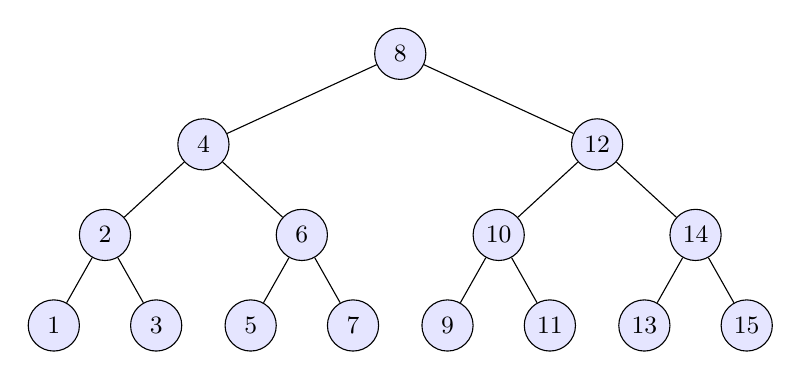
\begin{tikzpicture}[
  level distance=1.15cm,
  level 1/.style={sibling distance=5cm},
  level 2/.style={sibling distance=2.5cm},
  level 3/.style={sibling distance=1.3cm},
  every node/.style={circle, draw, fill=blue!10,
                     inner sep=1pt, minimum size=0.65cm, font=\small}
]
\node {8}
  child { node {4}
    child { node {2}
      child { node {1} }
      child { node {3} }
    }
    child { node {6}
      child { node {5} }
      child { node {7} }
    }
  }
  child { node {12}
    child { node {10}
      child { node {9} }
      child { node {11} }
    }
    child { node {14}
      child { node {13} }
      child { node {15} }
    }
  };
\end{tikzpicture}
\end{center}

% ══════════════════════════════════════════════
\subsection{Définition et propriété fondamentale}

\begin{definition}{Arbre binaire de recherche (ABR)}{bst}
Un \textbf{ABR} est un arbre binaire $T$ où chaque nœud $x$ vérifie :
\begin{itemize}[noitemsep]
  \item Si $y$ est dans le \emph{sous-arbre gauche} de $x$ :
        $y.\mathit{key} < x.\mathit{key}$.
  \item Si $y$ est dans le \emph{sous-arbre droit} de $x$ :
        $y.\mathit{key} \ge x.\mathit{key}$.
\end{itemize}
La \textbf{hauteur} $h$ est le nombre d'arêtes du plus long chemin racine–feuille.
\end{definition}

\begin{center}
\begin{tikzpicture}[font=\small]
  % Balanced BST
  \begin{scope}[
    level distance=0.9cm,
    level 1/.style={sibling distance=1.8cm},
    level 2/.style={sibling distance=0.9cm},
    every node/.style={circle, draw, fill=green!15,
                       inner sep=1pt, minimum size=0.6cm}]
    \node at (0,0) {8}
      child { node {4}
        child { node {2} }
        child { node {6} }
      }
      child { node {12}
        child { node {10} }
        child { node {14} }
      };
    \node[draw=none, fill=none, below=0.1cm, keygreen] at (0,-2.9)
          {Équilibré : $h = 2$, ops en $O(\log n)$};
  \end{scope}
  % Degenerate BST
  \begin{scope}[xshift=5.5cm,
    level distance=0.85cm,
    level 1/.style={sibling distance=1cm},
    every node/.style={circle, draw, fill=red!15,
                       inner sep=1pt, minimum size=0.6cm}]
    \node at (0,0) {2}
      child[missing]{}
      child { node {4}
        child[missing]{}
        child { node {6}
          child[missing]{}
          child { node {8} }
        }
      };
    \node[draw=none, fill=none, below=0.1cm, keyred] at (0.5,-2.9)
          {Dégénéré : $h = n-1$, ops en $O(n)$};
  \end{scope}
\end{tikzpicture}
\end{center}

\begin{complexity}{Toutes les opérations sur un ABR}{bstcplx}
Recherche, insertion, suppression, min, max, successeur, prédécesseur :
toutes en $O(h)$. Pour un arbre équilibré : $h = O(\log n)$.
\end{complexity}

% ══════════════════════════════════════════════
\subsection{Requêtes sur un ABR}

\subsubsection{Recherche}

\begin{algorithm}[H]
\caption{BST-Search($T$, $k$)}
\begin{algorithmic}[1]
\State $x \leftarrow T.\mathit{root}$
\While{$x \ne \textsc{NIL}$ \textbf{and} $k \ne x.\mathit{key}$}
  \If{$k < x.\mathit{key}$}  \State $x \leftarrow x.\mathit{left}$
  \Else                       \State $x \leftarrow x.\mathit{right}$
  \EndIf
\EndWhile
\State \Return $x$
\end{algorithmic}
\end{algorithm}

\subsubsection{Minimum, Maximum, Successeur}

\begin{theorem}{Localisation de min/max}{minmax}
\begin{itemize}[noitemsep]
  \item Le \textbf{minimum} est le nœud le plus à \emph{gauche}.
  \item Le \textbf{maximum} est le nœud le plus à \emph{droite}.
\end{itemize}
\end{theorem}

Le \textbf{successeur} de $x$ (plus petite clé $> x.\mathit{key}$) se trouve :
\begin{enumerate}[noitemsep]
  \item Si $x$ a un sous-arbre droit : c'est le \emph{minimum} du sous-arbre droit.
  \item Sinon : remonter jusqu'au premier ancêtre $y$ tel que $x$ est dans le sous-arbre
        \emph{gauche} de $y$.
\end{enumerate}

% ══════════════════════════════════════════════
\subsection{Parcours d'un ABR}

\begin{center}
\renewcommand{\arraystretch}{1.3}
\begin{tabular}{llll}
\toprule
\textbf{Parcours} & \textbf{Ordre} & \textbf{Résultat (ex.)} & \textbf{Utilité} \\
\midrule
Infixe (inorder)    & gauche, racine, droite & $1,2,\ldots,n$ (trié !) & Tri \\
Préfixe (preorder)  & racine, gauche, droite & racine en premier & Copie \\
Postfixe (postorder)& gauche, droite, racine & racine en dernier & Suppression \\
\bottomrule
\end{tabular}
\end{center}

\begin{remark}{Parcours infixe et tri}{inorder}
Le parcours infixe d'un ABR produit toujours les clés en \textbf{ordre croissant}
(propriété directe de la définition de l'ABR). Complexité : $\Theta(n)$.
\end{remark}

% ══════════════════════════════════════════════
\subsection{Modifications d'un ABR}

\subsubsection{Insertion}

Chercher $z.\mathit{key}$ jusqu'à atteindre \textsc{NIL}, puis insérer $z$ à cet endroit.
Complexité : $O(h)$.

\subsubsection{Suppression}

Trois cas selon le nombre d'enfants du nœud $z$ à supprimer :

\begin{center}
\begin{tikzpicture}[font=\small, >=Stealth,
    node/.style={circle, draw, fill=blue!10,
                 inner sep=1pt, minimum size=0.6cm}]
  % Case 1: no children
  \begin{scope}
    \node[node, fill=red!20] (z1) at (0,0) {$z$};
    \node[draw=none, below=5pt of z1] {\textit{Cas 1 : aucun enfant}};
    \node[draw=none, below=20pt of z1, font=\tiny] {Supprimer directement};
  \end{scope}
  % Case 2: one child
  \begin{scope}[xshift=3.5cm]
    \node[node] (p2) at (0,0.8) {$p$};
    \node[node, fill=red!20] (z2) at (0,0) {$z$};
    \node[node] (c2) at (0,-0.8) {$c$};
    \draw (p2)--(z2)--(c2);
    \draw[->, keygreen, thick] (p2) to[bend right=40] (c2);
    \node[draw=none, below=5pt of c2] {\textit{Cas 2 : un enfant}};
    \node[draw=none, below=25pt of c2, font=\tiny] {Remplacer $z$ par $c$};
  \end{scope}
  % Case 3: two children
  \begin{scope}[xshift=7.5cm,
    level distance=0.8cm,
    level 1/.style={sibling distance=1.2cm}]
    \node[node, fill=red!20] (z3) at (0,0) {$z$}
      child { node[node] {$\ldots$} }
      child { node[node] (succ) {$y$}
        child[missing]{}
        child { node[node] {$\ldots$} }
      };
    \node[above=2pt of succ, font=\tiny, keyblue] {successeur};
    \node[draw=none, below=0.3cm] at (0,-1.6) {\textit{Cas 3 : deux enfants}};
    \node[draw=none, below=1.5cm, font=\tiny, align=center] at (0,-1.6)
          {Remplacer $z$ par\\son successeur $y$};
  \end{scope}
\end{tikzpicture}
\end{center}

% ══════════════════════════════════════════════
\subsection{Bilan des opérations sur un ABR}

\begin{center}
\renewcommand{\arraystretch}{1.35}
\begin{tabular}{lcc}
\toprule
\textbf{Opération} & \textbf{Temps} & \textbf{Idée clé} \\
\midrule
Recherche              & $O(h)$      & Suivre gauche/droite selon la clé \\
Minimum / Maximum      & $O(h)$      & Nœud le plus à gauche/droite \\
Successeur / Préd.     & $O(h)$      & Min du s.a. droit, ou premier ancêtre \\
Insertion              & $O(h)$      & Phase de recherche + insertion feuille \\
Suppression            & $O(h)$      & 3 cas ; utilise \textsc{Transplant} \\
Parcours infixe        & $\Theta(n)$ & Visite chaque nœud une fois \\
\bottomrule
\end{tabular}
\end{center}

\begin{remark}{Équilibrage}{balance}
Dans le pire cas $h = \Theta(n)$ (arbre dégénéré). Les arbres auto-équilibrés
(AVL, rouge-noir) maintiennent $h = O(\log n)$, garantissant $O(\log n)$ par opération.
\end{remark}

% ══════════════════════════════════════════════
\subsection{Comparaison des structures de données}

\begin{center}
\renewcommand{\arraystretch}{1.4}
\begin{tabular}{lcccc}
\toprule
\textbf{Structure}   & \textbf{Capacité} & \textbf{Insertion} & \textbf{Suppression} & \textbf{Recherche} \\
\midrule
Pile / File (tableau)  & fixe    & $O(1)$       & $O(1)$       & $O(n)$ \\
Liste chaînée          & dynamique & $O(1)$     & $O(1)$       & $O(n)$ \\
ABR équilibré          & dynamique & $O(\log n)$ & $O(\log n)$ & $O(\log n)$ \\
\bottomrule
\end{tabular}
\end{center}

% ══════════════════════════════════════════════════════════════════════════════
\section*{Programmation Dynamique}
\addcontentsline{toc}{subsection}{Programmation Dynamique}
% ══════════════════════════════════════════════════════════════════════════════

\subsection{Paradigme et idée centrale}

\begin{definition}{Programmation dynamique (PD)}{dp}
La \textbf{programmation dynamique} est un paradigme algorithmique (pas une
fonctionnalité de langage). Son principe :
\begin{center}
  \textbf{Mémoriser les calculs déjà effectués pour éviter de les refaire.}
\end{center}
Cela permet de transformer des algorithmes exponentiels en algorithmes polynomiaux.
\end{definition}

Un algorithme DP repose sur deux propriétés :
\begin{enumerate}
  \item \textbf{Sous-structure optimale} : la solution optimale d'un problème contient les
        solutions optimales de ses sous-problèmes.
  \item \textbf{Sous-problèmes répétés} : un algorithme récursif naïf recalcule les mêmes
        sous-problèmes un nombre exponentiel de fois.
\end{enumerate}

\textbf{Deux stratégies d'implémentation :}
\begin{itemize}
  \item \textbf{Top-down avec mémoïsation} : récursion + table de résultats.
  \item \textbf{Bottom-up} : remplir la table des petits sous-problèmes vers les grands.
\end{itemize}

% ══════════════════════════════════════════════
\subsection{Premier exemple : nombres de Fibonacci}

\[
  F_0 = 1,\quad F_1 = 1,\quad F_n = F_{n-1} + F_{n-2} \quad (n \ge 2).
\]

\subsubsection{Récursion naïve : arbre de calcul exponentiel}

\begin{center}
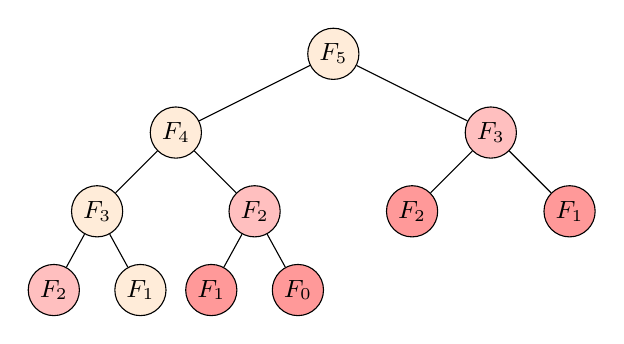
\begin{tikzpicture}[
    level distance=1cm,
    level 1/.style={sibling distance=4cm},
    level 2/.style={sibling distance=2cm},
    level 3/.style={sibling distance=1.1cm},
    every node/.style={circle, draw, fill=orange!15,
                       inner sep=1pt, minimum size=0.65cm, font=\small}
]
\node {$F_5$}
  child { node {$F_4$}
    child { node {$F_3$}
      child { node[fill=red!25] {$F_2$} }
      child { node {$F_1$} }
    }
    child { node[fill=red!25] {$F_2$}
      child { node[fill=red!40] {$F_1$} }
      child { node[fill=red!40] {$F_0$} }
    }
  }
  child { node[fill=red!25] {$F_3$}
    child { node[fill=red!40] {$F_2$} }
    child { node[fill=red!40] {$F_1$} }
  };
\end{tikzpicture}

\vspace{0.3em}
{\small \textcolor{keyred}{Les nœuds rouges sont recalculés plusieurs fois !}}
\end{center}

Complexité : \textbf{exponentielle} $O(2^n)$.

\subsubsection{Bottom-up DP : $\Theta(n)$}

\begin{algorithm}[H]
\caption{Bottom-Up-Fib($n$)}
\begin{algorithmic}[1]
\State $r[0] \leftarrow 1$;\; $r[1] \leftarrow 1$
\For{$i = 2$ \textbf{to} $n$}
  \State $r[i] \leftarrow r[i-1] + r[i-2]$
\EndFor
\State \Return $r[n]$
\end{algorithmic}
\end{algorithm}

\begin{center}
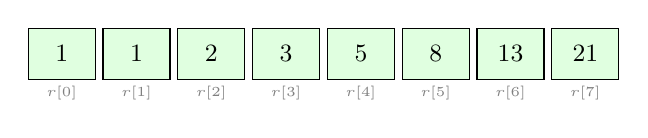
\begin{tikzpicture}[font=\small]
  \foreach \v/\i in {1/0, 1/1, 2/2, 3/3, 5/4, 8/5, 13/6, 21/7}{
    \node[draw, fill=green!12, minimum width=0.85cm, minimum height=0.65cm]
          at (\i*0.95, 0) {\v};
    \node[font=\tiny, gray] at (\i*0.95, -0.5) {$r[\i]$};
  }
\end{tikzpicture}
\end{center}

% ══════════════════════════════════════════════
\subsection{Coupe de tiges (\textit{Rod Cutting})}

\begin{definition}{Problème de la coupe de tiges}{rodcut}
\textbf{Entrée :} une tige de longueur $n$ et un tableau de prix $p_i$ pour une tige
de longueur $i$ ($1 \le i \le n$). \\
\textbf{Objectif :} trouver la découpe maximisant le revenu total.
\end{definition}

Il existe $2^{n-1}$ découpages possibles : la force brute est inenvisageable.

\subsubsection{Sous-structure optimale et récurrence}

\begin{theorem}{Structure optimale}{rodthm}
Si la première coupe optimale est après $i$ unités, et si
$s_1, \ldots, s_k$ est un découpage optimal de la tige restante de longueur $n-i$,
alors $i, s_1, \ldots, s_k$ est optimal pour la tige de longueur $n$.
\end{theorem}

Soit $r(n)$ le revenu optimal pour une tige de longueur $n$ :
\[
  r(n) =
  \begin{cases}
    0 & \text{si } n = 0, \\
    \displaystyle\max_{1 \le i \le n} \bigl\{ p_i + r(n-i) \bigr\} & \text{si } n \ge 1.
  \end{cases}
\]

\begin{center}
\begin{tikzpicture}[font=\small, >=Stealth]
  % Rod
  \draw[fill=brown!30, draw=brown!60!black] (0,-0.2) rectangle (6,0.2);
  \foreach \x in {1,2,3,4,5}{
    \draw[dashed, gray] (\x,-0.3) -- (\x,0.35);
  }
  \draw[keyred, very thick] (2,-0.35) -- (2,0.35)
        node[above, keyred, font=\tiny] {coupe après $i$};
  \draw[decorate, decoration={brace, amplitude=4pt}] (0,0.35) -- (2,0.35)
        node[midway, above=4pt] {$i$};
  \draw[decorate, decoration={brace, amplitude=4pt}] (2,0.35) -- (6,0.35)
        node[midway, above=4pt] {$n-i$ (sous-problème)};
\end{tikzpicture}
\end{center}

\begin{complexity}{DP pour la coupe de tiges}{rcplx}
\begin{itemize}[noitemsep]
  \item Top-down avec mémoïsation : $O(n^2)$ (graphe de sous-problèmes).
  \item Bottom-up : $O(n^2)$.
\end{itemize}
\end{complexity}

\subsubsection{Reconstruction de la solution}

On maintient un tableau $s[j]$ stockant la première coupe optimale pour $r(j)$.
Ensuite, on trace-back : couper $s[n]$, puis résoudre sur $n - s[n]$.

\[
\begin{array}{ccccccccc}
\toprule
i    & 0 & 1 & 2 & 3 & 4  & 5  & 6  & 7  & 8  \\
\midrule
r[i] & 0 & 1 & 5 & 8 & 10 & 13 & 17 & 18 & 22 \\
s[i] & 0 & 1 & 2 & 3 &  2 &  2 &  6 &  1 &  2 \\
\bottomrule
\end{array}
\]

% ══════════════════════════════════════════════
\subsection{Problème du rendu de monnaie}

\begin{definition}{Rendu de monnaie}{change}
\textbf{Entrée :} $n$ dénominations $0 < w_1 < \cdots < w_n$ et un montant cible $W$. \\
\textbf{Sortie :} nombre minimum de pièces pour atteindre exactement $W$.
\end{definition}

Récurrence DP :
\[
  c(w) =
  \begin{cases}
    0 & \text{si } w = 0, \\
    \displaystyle\min_{\substack{1 \le j \le n \\ w_j \le w}} \bigl\{1 + c(w - w_j)\bigr\}
       & \text{si } w \ge 1.
  \end{cases}
\]

\textbf{Exemple :} $w_1=1, w_2=2, w_3=5$, $W=8$.
Optimal : 1 pièce de chaque $\Rightarrow$ 3 pièces au total.

Remplissage bottom-up de $w=0$ à $W$ : complexité $O(nW)$.

% ══════════════════════════════════════════════
\subsection{Recette générale pour la PD}

\begin{tcolorbox}[colback=lightblue, colframe=keyblue,
                  title={\textbf{Étapes de conception d'un algorithme DP}},
                  fonttitle=\bfseries]
\begin{enumerate}
  \item \textbf{Identifier les choix et la sous-structure optimale} : un choix réduit
        le problème à de plus petits sous-problèmes, dont les solutions optimales
        composent la solution globale.
  \item \textbf{Écrire une récurrence} pour la valeur optimale en fonction des
        sous-problèmes.
  \item \textbf{Éviter les recalculs} via mémoïsation (top-down) ou remplissage
        de table (bottom-up).
  \item \textbf{(Optionnel) Reconstruire la solution} en stockant les choix dans une
        table auxiliaire et en remontant le tracé.
\end{enumerate}
\end{tcolorbox}

\begin{center}
\renewcommand{\arraystretch}{1.35}
\begin{tabular}{lcl}
\toprule
\textbf{Problème} & \textbf{Complexité} & \textbf{Taille de la table} \\
\midrule
Fibonacci         & $\Theta(n)$   & $n+1$ entrées \\
Coupe de tiges    & $O(n^2)$      & $n+1$ entrées \\
Rendu de monnaie  & $O(nW)$       & $W+1$ entrées \\
\bottomrule
\end{tabular}
\end{center}